% 图 61.4 —— 由 `checks/emit_hand.py` 自动拼出（probe 精测 + prims2 图元分解）
%%
% ⚠ 这是**稿子不是成品**：跑 `checks/checkhand.py 61.4` 看指标 + 看叠合图。
%%
%% ⚠ 待核：
%   · 本图 probe 报出阴影族 1 个 —— **本脚本不生成阴影**（要照原书手写）；prims2 的 strokes 里可能含阴影线，核对时留意别画重
%   · 可疑字形 1 项（空心圈 ⊙ 常被认成字母 o）—— 见文件末
%%
\documentclass[12pt]{standalone}
\usepackage{fontspec}
\setsansfont{Arial}
\newfontfamily\mfallback{DejaVu Sans}
\usepackage{tikz}
\begin{document}
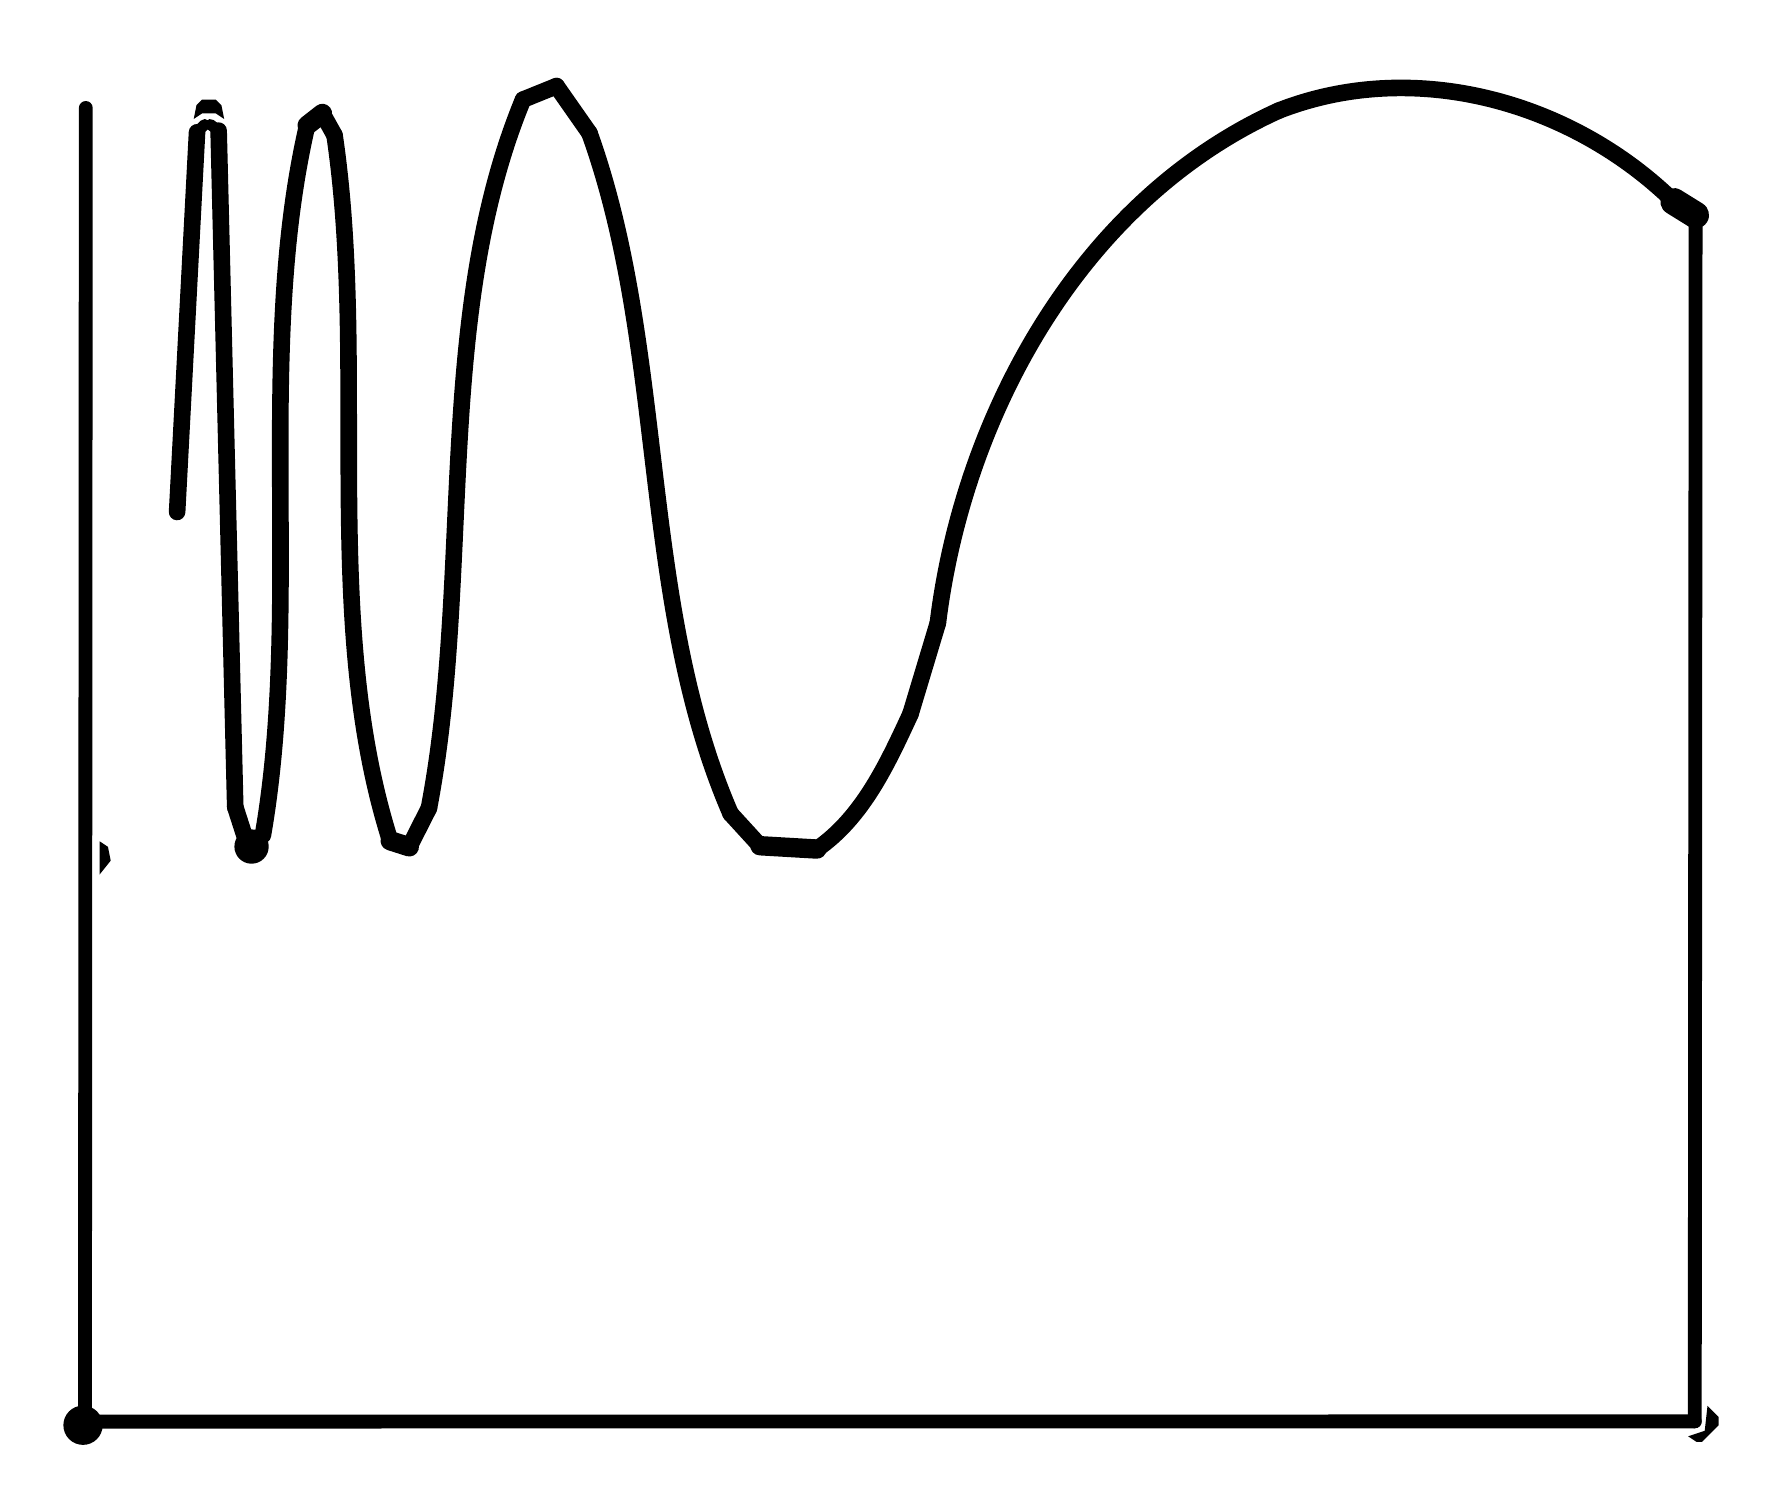
\begin{tikzpicture}[x=1pt, y=-1pt, line width=6.0pt, line cap=round, line join=round]

  %% ════ 填充区（prims2 的 fills）════
  \fill (61.0,28.0) -- (60.0,33.0) -- (63.0,31.0) -- (68.0,31.0) -- (71.0,33.0) -- (70.0,28.0) -- (68.0,26.0) -- (63.0,26.0) -- cycle;
  \fill (26.0,294.0) -- (26.0,306.0) -- (30.0,301.0) -- (29.0,296.0) -- cycle;
  \fill (607.0,498.0) -- (606.0,507.0) -- (600.0,509.0) -- (603.0,511.0) -- (605.0,511.0) -- (611.0,505.0) -- (611.0,502.0) -- cycle;

  %% ════ 直线段（prims2 的 strokes）════
  \draw[line width=6.0pt] (79.0,294.0) -- (75.0,281.6);
  \draw[line width=6.0pt] (75.0,281.6) -- (69.0,37.2);
  \draw[line width=4.0pt] (69.0,37.2) -- (66.0,35.0);
  \draw[line width=4.8pt] (81.0,294.0) -- (85.0,291.8);
  \draw[line width=7.0pt] (101.0,35.3) -- (106.5,31.0);
  \draw[line width=6.0pt] (106.5,31.0) -- (110.9,38.9);
  \draw[line width=7.0pt] (131.0,293.8) -- (137.9,296.0);
  \draw[line width=6.0pt] (137.9,296.0) -- (145.0,282.0);
  \draw[line width=6.0pt] (179.0,26.0) -- (191.1,21.1);
  \draw[line width=6.0pt] (191.1,21.1) -- (203.0,38.1);
  \draw[line width=6.0pt] (254.0,284.0) -- (264.6,295.6);
  \draw[line width=7.0pt] (264.6,295.6) -- (285.2,296.8);
  \draw[line width=6.0pt] (319.0,248.0) -- (328.9,215.1);
  \draw[line width=9.7pt] (594.8,62.8) -- (602.7,67.7);
  \draw[line width=5.0pt] (602.7,67.7) -- (602.4,503.6);
  \draw[line width=5.0pt] (602.4,503.6) -- (20.7,503.7);
  \draw[line width=5.0pt] (20.7,503.7) -- (21.0,29.0);
  \draw[line width=6.0pt] (54.0,175.0) -- (61.2,37.8);
  \draw[line width=4.0pt] (61.2,37.8) -- (64.0,35.0);

  %% ════ 曲线（prims2 的 curves —— 三段式，坐标同为 (y,x)）════
  \draw[line width=6.0pt] (85.0,291.8) .. controls (99.3,209.0) and (82.1,117.1) .. (101.0,35.3);
  \draw[line width=6.0pt] (110.9,38.9) .. controls (123.2,122.8) and (105.7,214.1) .. (131.0,293.8);
  \draw[line width=6.0pt] (145.0,282.0) .. controls (161.0,198.2) and (146.6,104.5) .. (179.0,26.0);
  \draw[line width=6.0pt] (203.0,38.1) .. controls (231.2,116.6) and (220.8,207.4) .. (254.0,284.0);
  \draw[line width=6.0pt] (285.2,296.8) .. controls (301.9,285.2) and (310.7,265.9) .. (319.0,248.0);
  \draw[line width=6.0pt] (328.9,215.1) .. controls (338.0,140.7) and (380.0,62.6) .. (452.0,30.0);
  \draw[line width=6.0pt] (452.0,30.0) .. controls (501.0,10.8) and (557.8,26.6) .. (594.8,62.8);

  %% ════ 实心点 ════
  \fill (80.9,295.9) circle (6.2);
  \fill (20.0,505.0) circle (7.1);

  %% ════ 标签（probe 直接给的 \node 行）════
  %% ⚠ 全部补了 fill=white：文字在最上层，否则与曲线交叉干扰

  % 钉死画布：否则超出的图元/控制点会把页面撑大，1:1 回比就失准
  \pgfresetboundingbox
  \path[use as bounding box] (0,0) rectangle (621,521);
\end{tikzpicture}
\end{document}

% ⚠ 待核清单（probe 拿不准，人眼过一遍）：
%   · 未识别/跳过：⑤ 跳过/未识别的字形
